\documentclass[
  11pt,
  letterpaper,
   addpoints,
   answers
  ]{exam}

\usepackage{../exercise-preamble}
\usepackage{float}

\begin{document}

\noindent
\begin{minipage}{0.47\textwidth}

\includegraphics[width=\textwidth]{../fcfm_die}
\end{minipage}
\begin{minipage}{0.53\textwidth}
\begin{center} 
\large\textbf{Análisis de Sistemas Dinámicos y Estimación} (EL3204-1) \\
\large\textbf{Clase auxiliar 1} \\
\normalsize Prof.~ Marcos Orchard - Sebastián Espinosa.\\
\normalsize Prof.~Aux.~Erik Sáez
\end{center}
\end{minipage}

\vspace{0.5cm}
\noindent
\vspace{.85cm}

\begin{questions}
    %%%%%%%%%%%%%%%%%%%%%%%%%%%
    \question Considere el sistema de la siguiente figura, donde se tiene un carro atado a un resorte con un sensor de distancia, capaz de medir la distancia del carro a la pared. Suponga que existe una fuerza de fricción viscosa con la superficie $F_f$ de la forma $F_f = b_1 \dot{z} + b_2 (\dot{z}^2)$.
    \begin{figure}[ht]
        \centering
        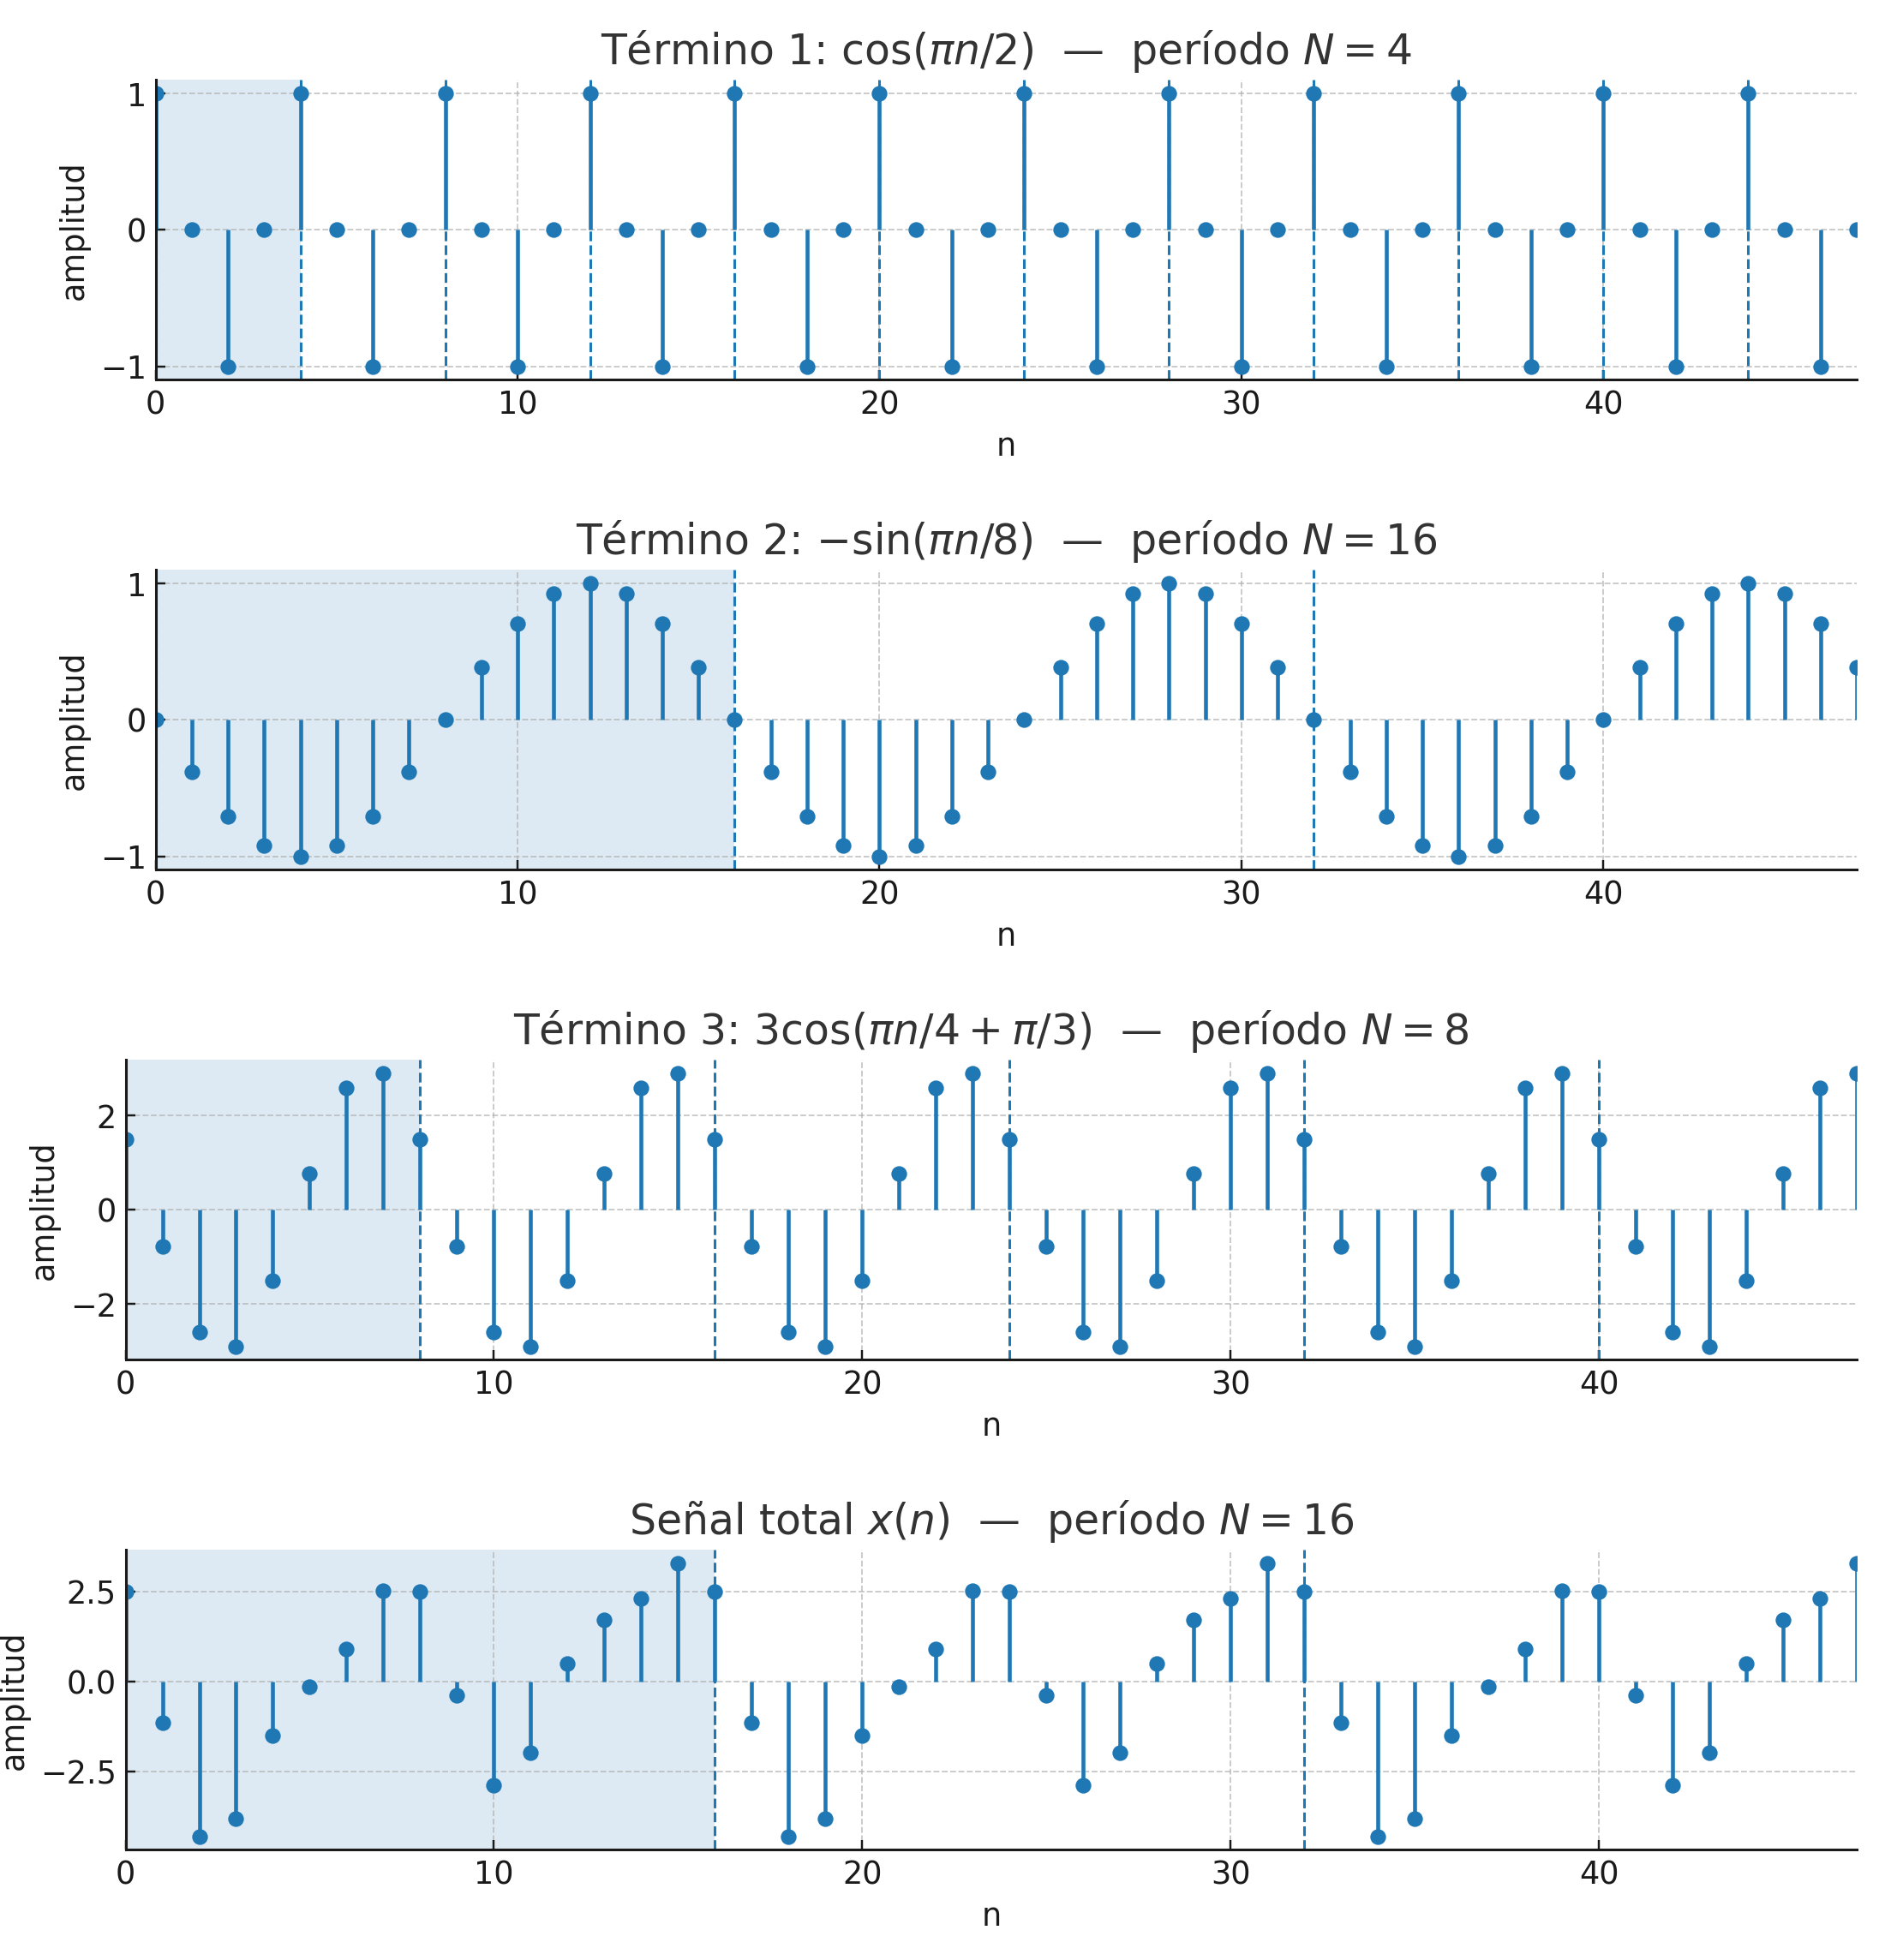
\includegraphics[width=0.45\textwidth]{Auxiliar_1_1}
    \end{figure}
    \begin{enumerate}
        \item Establezca hipótesis simplificatorias para el problema.
        \item Formule un modelo matemático del sistema que sea consistente con sus hipótesis.
        \item Encuentre el punto de operación que asegure $z = 1$ m.
    \end{enumerate}
    %%%%%%%%%%%%%%%%%%%%%%%%%%%
    \begin{solution}
    \subsection*{Resolución 1.1}
        Para poder plantear un buen modelo, es necesario establecer hipótesis que simplifiquen el problema y lo hagan abordable. Estas hipótesis son muy importantes, ya que pueden complejizar o simplificar el problema cuanto sea necesario. Para este caso particular, algunas hipótesis que se pueden plantear para simplificar el problema son:
\begin{enumerate}
    \item El carro solamente se mueve \textbf{horizontalmente.}
    \item El resorte actúa en el \textbf{régimen lineal}, de acuerdo a la ley de Hooke.
    \item La constante elástica $k$ del resorte no varía, y su largo natural $l_0$ es 0.
    \item La fricción es de la forma 
    \begin{equation}
        F_f = b_1 \dot{z} + b_2 \dot{z}^2.
    \end{equation}
    \item La fuerza $F(t)$ es conocida y varía en el tiempo.
\end{enumerate}
\subsection*{Resolución 1.2}
Plantear un modelo matemático para un sistema físico se reduce, generalmente, a encontrar una ecuación diferencial que modele la dinámica del sistema. Para este caso particular, podemos utilizar la segunda ley de Newton para obtener dicha ecuación diferencial (esto es una de las tantas formas posibles de abordar el problema).
\begin{equation}
    m\ddot{z} = F(t) - F_e - F_f, 
\end{equation}
Donde $F_e$ corresponde a la fuerza elástica del resorte y $F_f$ es la fuerza de fricción. La fuerza elástica, debido a la segunda hipótesis (\textit{$l_{0}=0$}), estará dada por:
\begin{equation}
    F_e = kz, 
\end{equation}
por lo que la ecuación anterior es
\begin{equation}
    m\ddot{z} = F(t) - kz - b_1\dot{z} - b_2\dot{z}^2. 
\end{equation}
Despejando $\ddot{z}$, tenemos que el modelo matemático es
\begin{equation}
    \ddot{z} = \frac{1}{m}F(t) - \frac{k}{m}z - \frac{b_1}{m}\dot{z} - \frac{b_2}{m}\dot{z}^2. 
\end{equation}
Sabemos que este será el modelo matemático, ya que captura la dinámica del sistema en función de las fuerzas actuantes y las propiedades del resorte. 
\subsection*{Resolución 1.3}
Para encontrar el punto de operación, el objetivo es determinar el valor de la entrada $F(t)$ de modo tal que se tenga $z = 1 \, \text{m}$. Implícitamente, al hablar de punto de operación se requiere estaticidad (a menos que se indique lo contrario), por lo que podemos asumir que $z$ no varía, indicando que $\dot{z} = \ddot{z} = 0$.

Podemos utilizar lo anteriormente mencionado sobre el modelo, imponiendo las condiciones indicadas y encontrando el valor de $F(t)$ que las satisfaga. Imponiendo $z = 1$, $\dot{z} = \ddot{z} = 0$ sobre la ecuación anterior, tenemos:
\begin{equation}
    0 = \frac{1}{m}F(t) - \frac{k}{m} \cdot 1 \quad \Rightarrow \quad F(t) = k,
\end{equation}
por lo que el punto de operación es $F(t) = k$. Un aspecto importante a considerar es que, para encontrar este punto de operación, asumimos que la fuerza $F(t)$ es constante en el tiempo. Más adelante en el curso (y en otros cursos de la carrera) veremos que considerar una fuerza constante no siempre es lo ideal, sino que es posible diseñar una entrada particular para alcanzar la condición de estaticidad más rápidamente.
    \end{solution}
    %%%%%%%%%%%%%%%%%%%%%%%%%%%
    \question Considere el siguiente péndulo apoyado en un carro móvil, el cual se desliza por una barra.
    \begin{enumerate}
        \item Establezca hipótesis simplificatorias.
        \item Formule un modelo matemático, que capture la dinámica del sistema.
        \item Identifique entradas, salidas y estados en su modelo.
        \item Linealice en torno a $\theta = \pi$.
    \end{enumerate}
    \begin{figure}[ht]
        \centering
        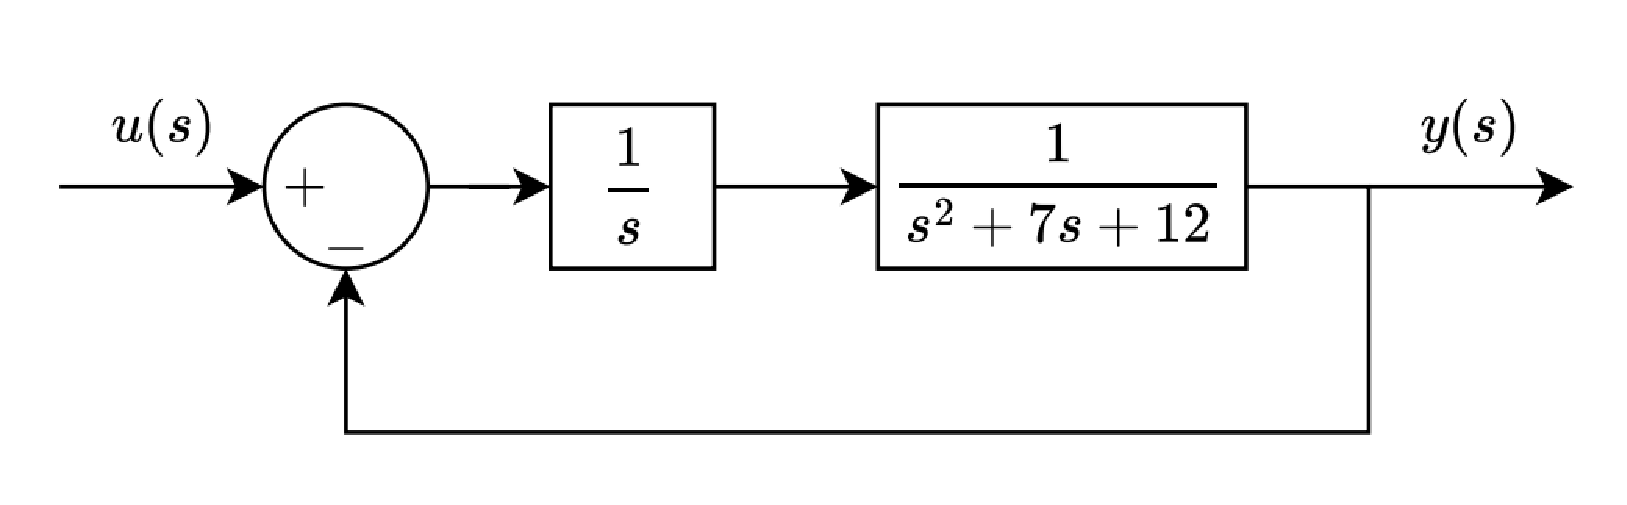
\includegraphics[width=0.5\textwidth]{Auxiliar_1_2}
    \end{figure}
%%%%%%%%%%%%%%%%%%%%%%%%%%%
\begin{solution}
\subsection*{Resolución 2.1}
    Primeramente, es necesario establecer buenas hipótesis simplificatorias para que el problema sea abordable. Algunas de estas hipótesis que podemos plantear son las siguientes:
\begin{enumerate}
    \item El carro tiene masa despreciable.
    \item La vara del péndulo no tiene masa.
    \item La vara del péndulo es rígida.
    \item La bola del péndulo es una masa puntual.
    \item No hay roce con el aire.
    \item Solamente existe movimiento en los dos ejes ilustrados.
\end{enumerate}
\subsection*{Resolución 2.2}
Utilizando las hipótesis planteadas, podemos encontrar un modelo matemático. Para esto, si bien se podría utilizar la segunda ley de Newton para plantear una ecuación diferencial, al ser un péndulo este es un proceso engorroso: en cambio, utilizaremos mecánica lagrangiana para plantear la ecuación diferencial. El lagrangiano corresponde a $L = T - V$, con $T$ la energía cinética y $V$ la energía potencial, junto a la ecuación de Euler-Lagrange
\begin{equation}
    \frac{\partial L}{\partial q} - \frac{d}{dt} \left( \frac{\partial L}{\partial \dot{q}} \right) = 0
\end{equation}
Es importante destacar que (\textbf{q}) representa la coordenada que estemos utilizando y por tanto dependerá también del sistema de coordenadas que se utilice. Además, la ecuación de Euler-Lagrange planteada de esa manera es válida si no existen pérdidas de energía en el sistema: si hubiesen fuerzas no conservativas, se deberían considerar dentro de la ecuación. Este supuesto es válido debido a la hipótesis de que no hay fricción. Para calcular el Lagrangiano, debemos comenzar calculando la energía cinética. Dado que solamente la bola del péndulo tiene masa, este será el único componente con energía cinética. Si llamamos $x_p, y_p$ a la posición del péndulo, podemos notar que esta se puede escribir como
\begin{equation}
    x_p = x + l \sin \theta \quad y_p = -l \cos \theta,
\end{equation}
Donde deberemos definir el sistema de referencia el cual se asume que $y$ es positivo hacia arriba, que $y = 0$ corresponde a la ubicación de la barra, y que se tiene una distancia $x(t)$ desde el origen a la vertical del péndulo. Con estas posiciones, la energía cinética estará dada por:
\begin{equation}
    T = \frac{1}{2} m \left( \dot{x}_p^2 + \dot{y}_p^2 \right). 
\end{equation}
 Dado que necesitamos las derivadas para el cálculo anterior, tenemos
\begin{equation}
    \dot{x}_p = \dot{x} + l \dot{\theta} \cos \theta \quad \dot{y}_p = l \dot{\theta} \sin \theta
\end{equation}
donde los términos $\dot{\theta}$ salen por la regla de la cadena (\textit{Es muy importante tener en consideración esto último, dado que $\dot{\theta}$ depende del tiempo, que es respecto a lo que estamos derivando}). Utilizándolos para calcular la energía cinética, tenemos:
\begin{equation}
    T = \frac{1}{2} m \left( \dot{x}^2 + 2 \dot{x} l \dot{\theta} \cos \theta + l^2 \dot{\theta}^2 \cos^2 \theta + l^2 \dot{\theta}^2 \sin^2 \theta \right)
\end{equation}
Podemos notar que:
\begin{equation}
    l^2 \dot{\theta}^2 \cos^2 \theta + l^2 \dot{\theta}^2 \sin^2 \theta = l^2 \dot{\theta}^2 (\cos^2 \theta + \sin^2 \theta) = l^2 \dot{\theta}^2
\end{equation}
Luego:
\begin{equation}
    T = \frac{1}{2} m \left( \dot{x}^2 + 2 \dot{x} l \dot{\theta} \cos \theta + l^2 \dot{\theta}^2 \right) = \frac{1}{2} m \dot{x}^2 + m l \dot{x} \dot{\theta} \cos \theta + \frac{1}{2} m l^2 \dot{\theta}^2. 
\end{equation}
Para la energía potencial, dado que el único componente que tiene masa es la bola del péndulo, solamente se tiene la contribución de su energía potencial gravitatoria. Además, dado que la vara es rígida, sabemos que no actúa como un resorte y, por ende, no hay energía potencial elástica. Considerando todo esto, la energía potencial $V$ está dada por
\begin{equation}
    V = mg \cdot y_p = -mgl \cos \theta. 
\end{equation}
Luego, el lagrangiano es
\begin{equation}
    L = \frac{1}{2} m \left( \dot{x}^2 + 2 \dot{x} l \dot{\theta} \cos \theta + l^2 \dot{\theta}^2 \right) + mgl \cos \theta. 
\end{equation}
Para poder considerar el Lagrangiano dentro de la ecuación de Euler-Lagrange, es necesario calcular las derivadas de cada término. Dado que estamos trabajando en coordenadas polares, sabemos que hay dos coordenadas, el radio \(r\) y el ángulo \(\theta\). Dado que \(r = l\) es constante, sabemos que no hay dinámica en la dirección radial, por lo que solamente nos interesa analizar la dinámica angular. Esto significa que debemos calcular las derivadas de \(L\) con respecto a \(\theta\) y \(\dot{\theta}\). Calculando las derivadas, tenemos
\begin{align}
    \frac{\partial L}{\partial \theta} &= -mgl \,\sin \theta \;-\; ml\,\dot{x}\,\dot{\theta}\,\sin \theta, \\
    \frac{\partial L}{\partial \dot{\theta}} &= ml^2\,\dot{\theta} \;+\; ml\,\dot{x}\,\cos \theta.
\end{align}
Un punto importante a notar a la hora de calcular las derivadas es que, al derivar respecto a $\theta$, se debe tener en cuenta que $\dot{\theta}$ no depende de $\theta$, sino solamente del tiempo. Lo mismo aplica a la hora de derivar respecto a $\dot{\theta}$, donde $\dot{\theta}$ actúa como una constante.
Luego, usando la ecuación 21 podemos tomar la derivada con respecto al tiempo, de lo que tenemos
\begin{align}
    \frac{d}{dt} \left( \frac{\partial L}{\partial \dot{\theta}} \right) 
    &= \frac{d}{dt} \left( ml^2 \dot{\theta} + ml \dot{x} \cos \theta \right) \tag{22}\\
    &= ml^2 \ddot{\theta} + ml \left( \ddot{x} \cos \theta - \dot{x} \dot{\theta} \sin \theta \right) \\
    &= ml^2 \ddot{\theta} + ml \ddot{x} \cos \theta - ml \dot{x} \dot{\theta} \sin \theta.
\end{align}
Insertando estos términos dentro de la ecuación de Euler--Lagrange, tenemos
\begin{align}
    \frac{\partial L}{\partial \theta} - \frac{d}{dt} \left( \frac{\partial L}{\partial \dot{\theta}} \right) &= 0 \\
    &= \left[ -mgl \sin \theta - ml\,\dot{x}\,\dot{\theta}\,\sin \theta \right] 
       - \left[ ml^2 \ddot{\theta} + ml\,\ddot{x} \cos \theta - ml\,\dot{x}\,\dot{\theta}\,\sin \theta \right] \\
    &= -mgl \sin \theta - ml^2 \ddot{\theta} - ml\,\ddot{x} \cos \theta = 0. 
\end{align}
Reordenando términos para despejar \(\ddot{\theta}\) en función del resto de variables, obtenemos
\begin{equation}
    \ddot{\theta} = -\frac{g}{l} \sin \theta - \frac{\cos \theta}{l} \,\ddot{x}, 
\end{equation}
la cual corresponde a la ecuación diferencial que modela la dinámica del problema.
\subsection*{Resolución 2.3}
Para identificar las entradas, debemos identificar aquellas variables que podemos manipular y que no dependen de la dinámica del problema. En este caso, podemos ver que $\ddot{x}$, correspondiente a la aceleración del carro, es una variable libre del problema, la cual no depende del resto de variables, por lo que podemos considerarla como la entrada al sistema.\\
Con respecto a la salida, esta es la variable que más libertad entrega a quien modela, dado que depende del fenómeno de interés. En general, se puede considerar como variable de salida cualquiera de los sensores que se están utilizando para medir las variables, por lo que estos valores medidos por los sensores podrían considerarse las salidas. Sin embargo, en este problema no se indican los sensores presentes, por lo que asumiremos que cualquier variable es salida, por lo que, arbitrariamente, se escoge que $\theta$ es la salida.\\
Finalmente, las últimas variables a indicar son los estados. Los estados corresponden a aquellas variables que tienen incidencia directa sobre la dinámica del sistema planteado. Una forma práctica de verlo es que cualquier diferencial que modele al sistema: si el sistema está modelado por una EDO de orden n, entonces todas las derivadas de menor orden (incluyendo el orden 0, que corresponde a la variable sin derivar) van a corresponder a los estados del sistema\footnote{Otra forma útil de verlo es que los estados van a corresponder a todas aquellas variables para las cuales se debe indicar una condición inicial.}. En el problema planteado, dado que el modelo es una EDO de orden 2, sabemos que las derivadas de orden 1 ($\dot{\theta}$) y orden 0 ($\theta$) serían los estados del sistema.
\subsection*{Resolución 2.4}
La linealización es un proceso en el cual generamos una aproximación lineal de la EDO que modela al sistema, utilizando los primeros términos de la serie de Taylor.
Para esto, notemos que podemos escribir la ecuación (29) como
\begin{equation}
    \ddot{\theta} = f(\theta, u),
\end{equation}
tal que
\begin{equation}
    f(\theta, u) = -\frac{g}{l} \sin \theta - \frac{\cos \theta}{l} u,
\end{equation}
donde hemos denotado $u = \ddot{x}$ para abreviar. 

La idea de linealizar es calcular la serie de Taylor de la función $f(\theta, u)$ en torno a un cierto punto $(\bar{\theta}, \bar{u})$, de modo que el sistema linealizado sea una \textbf{buena aproximación del sistema original en torno a dicho punto}.

Calculando la serie de Taylor de $f(\theta, u)$ en torno a $(\bar{\theta}, \bar{u})$ y omitiendo términos de orden superior, tenemos:
\begin{equation}
    f(\theta, u) \approx f(\bar{\theta}, \bar{u}) 
    + (\theta - \bar{\theta}) \frac{\partial f(\bar{\theta}, \bar{u})}{\partial \theta} 
    + (u - \bar{u}) \frac{\partial f(\bar{\theta}, \bar{u})}{\partial u}.
\end{equation}

Definimos las variables perturbadas:
\begin{equation}
    \tilde{\theta} := \theta - \bar{\theta}, 
    \qquad 
    \tilde{u} := u - \bar{u},
\end{equation}
y considerando que $\ddot{\theta} = f(\theta, u)$ y $\tilde{\ddot{\theta}} := \ddot{\theta} - f(\bar{\theta}, \bar{u})$, obtenemos:
\begin{equation}
    \tilde{\ddot{\theta}} = f_{\theta}(\bar{\theta}, \bar{u}) \, \tilde{\theta} 
    + f_{u}(\bar{\theta}, \bar{u}) \, \tilde{u}.
\end{equation}

Donde, para abreviar, definimos:
\begin{align}
    f_{\theta} &:= \frac{\partial f(\bar{\theta}, \bar{u})}{\partial \theta} 
    = -\frac{g}{l} \cos \bar{\theta} + \frac{\sin \bar{\theta}}{l} \, \bar{u}, \\
    f_{u} &:= \frac{\partial f(\bar{\theta}, \bar{u})}{\partial u} 
    = -\frac{\cos \bar{\theta}}{l}.
\end{align}

Evaluando en $(\bar{\theta}, \bar{u}) = (\pi, 0)$:
\begin{align}
    f_{\theta}(\pi, 0) &= -\frac{g}{l} \cos \pi + \frac{\sin \pi}{l} \cdot 0 
    = -\frac{g}{l}(-1) + 0 
    = \frac{g}{l}, \\
    f_{u}(\pi, 0) &= -\frac{\cos \pi}{l} 
    = -\frac{-1}{l} 
    = \frac{1}{l}.
\end{align}

Por lo tanto, el modelo linealizado en torno a \(\theta = \pi\) y \(u = 0\) es:
\begin{equation}
    \tilde{\ddot{\theta}} = \frac{g}{l} \, \tilde{\theta} + \frac{1}{l} \, \tilde{u}.
\end{equation}
Con lo que finalmente se obtiene el modelo linealizado.
\end{solution}
%%%%%%%%%%%%%%%%%%%%%%%%%%%
\question Considere el siguiente estanque cónico:
\begin{figure}[ht]
    \centering
    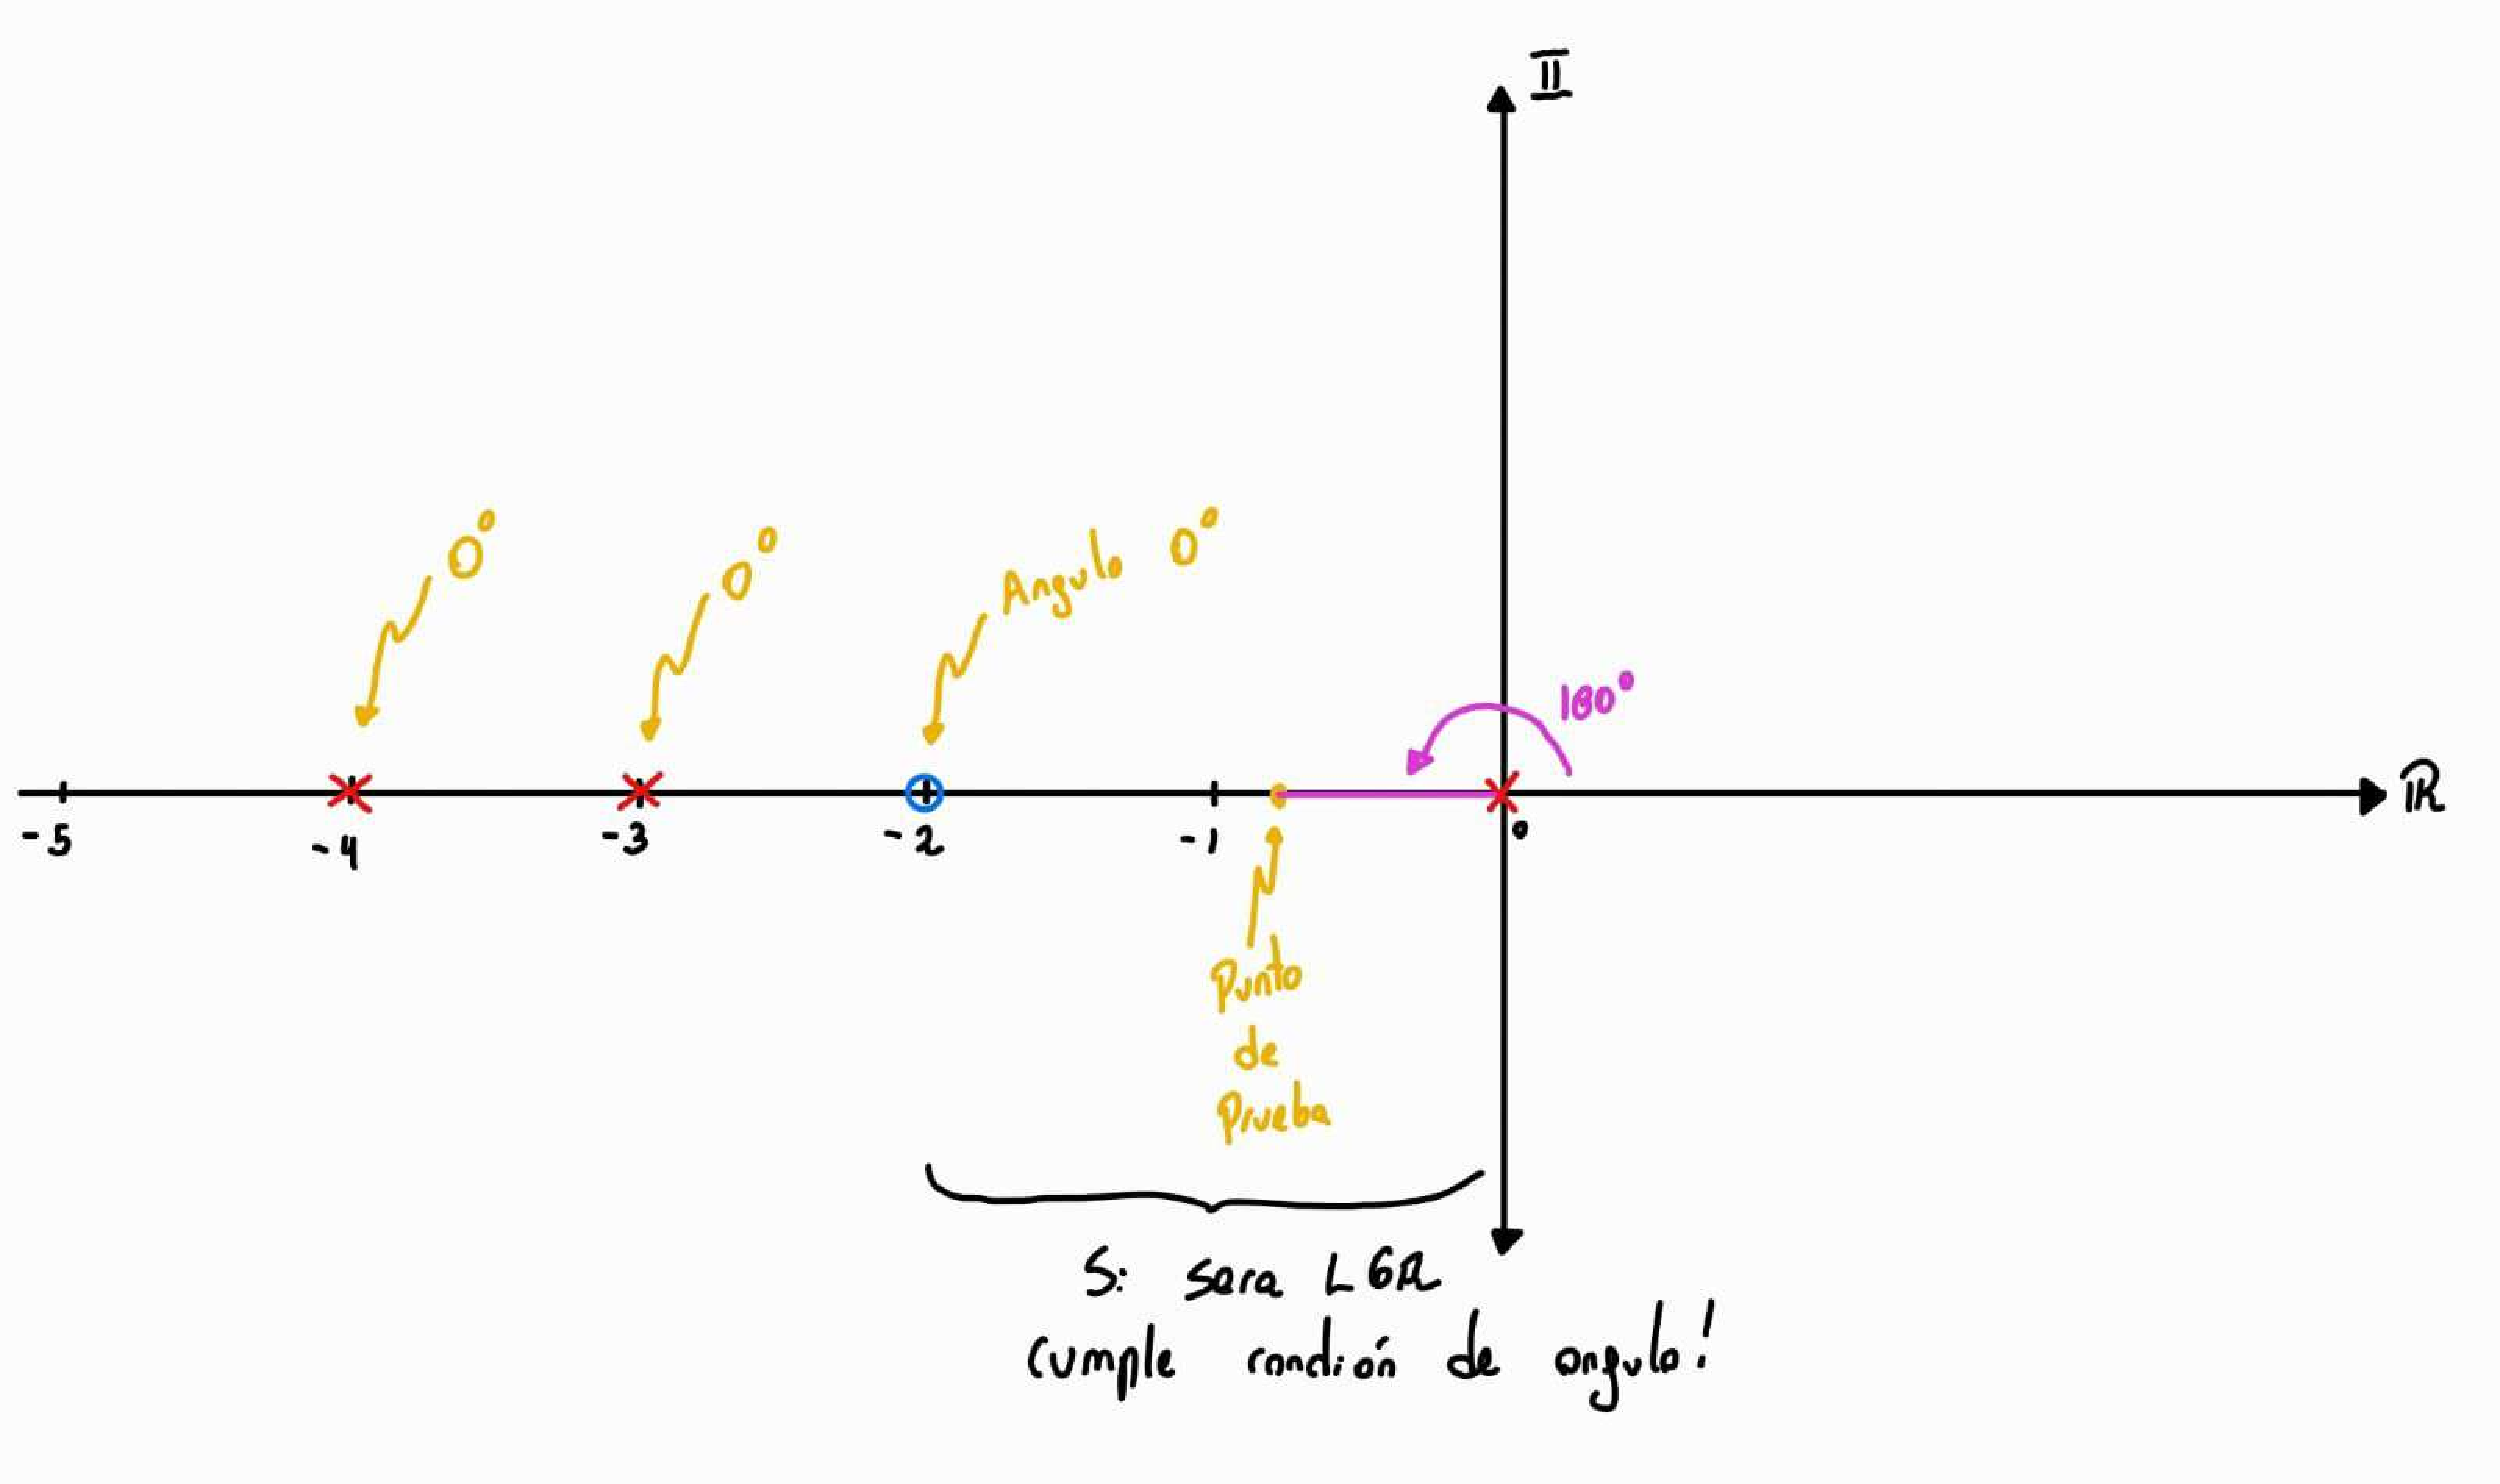
\includegraphics[width=0.4\textwidth]{Auxiliar_1_5}
    \caption{Estanque cónico}
\end{figure}

Se tienen los siguientes datos:
\begin{itemize}
    \item Altura máxima: $H = 8 \, \text{m}$
    \item Radio máximo: $R = 3 \, \text{m}$
    \item Volumen del estanque en función de la altura:
    \begin{equation}
        V(h) = \frac{\pi r^2 h}{3}, \tag{1}
    \end{equation}
    \item Flujo volumétrico de entrada: $F_1(t)$ (arbitrario)
    \item Flujo volumétrico de salida:
    \begin{equation}
        F(t) = \alpha \sqrt{h(t)}
    \end{equation}
    donde $\alpha$ corresponde a la apertura del canal. Para este ejercicio, considere $\alpha = 1$.
\end{itemize}

Responda lo siguiente:
\begin{enumerate}
    \item Encuentre un modelo dinámico no lineal que relacione la altura del agua $h(t)$ y el flujo de entrada $F_1(t)$, indicando claramente las hipótesis simplificatorias que tome.

    \item Linealice su modelo en torno a $h_0 = 4\,\text{m}$, $F_{1,0} = 2\,\text{m}^3/\text{s}$, y plantee una nueva ecuación diferencial lineal para el modelo perturbado, considerando:
    \begin{align*}
        h(t) &= h_0 + \Delta h(t) \\
        F_1(t) &= F_{1,0} + \Delta F_1(t)
    \end{align*}
    que relacione la salida del sistema linealizado $\Delta h(t)$ con la entrada del sistema linealizado $\Delta F_1(t)$. Para esto, al linealizar puede considerar que los términos de orden superior (por ejemplo, $\Delta h^2$, $\Delta F_1^2$, etc.) son despreciables y pueden anularse.
\end{enumerate}
%%%%%%%%%%%%%%%%
\begin{solution}
\subsection*{Resolución 3.1}
Dado que se busca plantear un modelo dinámico no lineal, es necesario establecer hipótesis simplificatorias adecuadas. Algunas que podemos considerar son las siguientes:
\begin{itemize}
    \item El estanque es un cono perfecto.
    \item No existen pérdidas de agua ni entradas adicionales al sistema.
    \item La velocidad del agua es lo suficientemente baja como para despreciar efectos inerciales.
    \item La superficie libre del agua es plana en todo momento.
    \item \ldots
\end{itemize}

La variación del volumen de agua en el estanque está determinada por la diferencia entre el flujo volumétrico de entrada y el flujo volumétrico de salida:
\begin{equation}
    \frac{dV}{dt} = F_1(t) - F(t).
\end{equation}

Recordando que el volumen de un cono está dado por:
\begin{equation}
    V(h) = \frac{\pi r^2 h}{3},
\end{equation}
observamos que el radio \(r(t)\) también depende del tiempo. Para relacionar \(r(t)\) con \(h(t)\) utilizamos el Teorema de Tales, considerando la geometría del estanque:

\begin{center}
    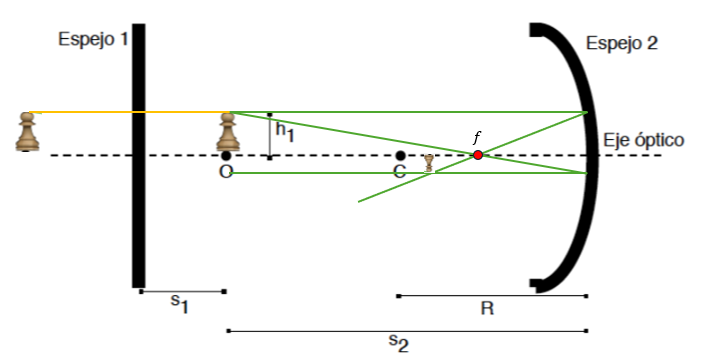
\includegraphics[width=0.2\textwidth]{Auxiliar_1_6}
\end{center}

De este modo:
\begin{align}
    \frac{r(t)}{h(t)} = \frac{R}{H} 
    \quad \Rightarrow \quad 
    r(t) = \frac{R}{H} \, h(t).
\end{align}

Sustituyendo en la expresión del volumen, se obtiene:
\begin{align}
    V(h) &= \frac{\pi \left( \frac{R}{H} h \right)^2 h}{3} 
    = \frac{\pi R^2}{3 H^2} h^3.
\end{align}

Derivando respecto del tiempo y usando la ecuación de balance de volúmenes:
\begin{align}
    \frac{dV}{dt} &= F_1(t) - F(t) \\
    \frac{d}{dt} \left( \frac{\pi R^2}{3 H^2} h^3 \right) = F_1(t) - F(t), \\
    \frac{\pi R^2}{H^2} h^2 \dot{h} &= F_1(t) - F(t).
\end{align}

Definiendo:
\begin{equation}
    k := \frac{\pi R^2}{H^2},
\end{equation}
y considerando que el flujo de salida está dado por \(F(t) = \alpha \sqrt{h(t)}\), se obtiene:
\begin{align}
    \dot{h} = \frac{1}{k\, h^{2}} \left[ F_1(t) - \alpha \sqrt{h(t)} \right].
\end{align}

Se observa que este modelo es claramente no lineal, ya que la ecuación diferencial contiene términos $\frac{1}{h^2}$ y $\sqrt{h}$.

   \subsection*{Resolución 3.2}
Se comienza considerando el modelo no lineal obtenido anteriormente:
\begin{equation}
    \dot h \;=\; f(h,F_1) \;=\; \frac{F_1 - \sqrt{h}}{k\,h^2},
    \qquad k := \frac{\pi R^2}{H^2},
\end{equation}
con el punto de operación dado por el enunciado:
\begin{equation}
    h_0 = 4\,\text{m}, 
    \qquad F_{1,0} = 2\,\text{m}^3/\text{s},
    \qquad \alpha=1,
\end{equation}
el cual satisface $0 = \frac{F_{1,0}-\sqrt{h_0}}{k h_0^2}$ (i.e., $F_{1,0}=\sqrt{h_0}=2$). Con lo que sabemos que es un punto de equilibrio. Luego se definen las perturbaciones:
\begin{equation}
    \Delta h := h - h_0,
    \qquad
    \Delta F_1 := F_1 - F_{1,0},
    \qquad
    \Delta \dot h := \dot h - \dot h_0 =\dot h.
\end{equation}

Linealizamos por serie de Taylor de $f(h,F_1)$ en $(h_0,F_{1,0})$:
\begin{equation}
    \Delta \dot h 
    \;=\; 
    \left.\frac{\partial f}{\partial h}\right|_{0}\,\Delta h
    \;+\;
    \left.\frac{\partial f}{\partial F_1}\right|_{0}\,\Delta F_1 .
\end{equation}
Sea $f(h,F_1) = \dfrac{F_1 - \sqrt{h}}{k\,h^2}$. Entonces
\begin{align}
    \frac{\partial f}{\partial h}
    &= \frac{1}{k}\,\frac{\partial}{\partial h}\!\left[(F_1-\sqrt{h})\,h^{-2}\right] \nonumber\\
    &= \frac{1}{k}\left[ -\frac{1}{2}h^{-1/2}\,h^{-2} \;+\; (F_1-\sqrt{h})(-2)h^{-3}\right],\\[0.25em]
    \frac{\partial f}{\partial F_1}
    &= \frac{1}{k}\,h^{-2}.
\end{align}
Evaluando en el punto de operación $(h_0,F_{1,0})=(4,2)$ (nótese que $F_{1,0}-\sqrt{h_0}=0$):
\begin{align}
    \left.\frac{\partial f}{\partial h}\right|_0
    &= \frac{1}{k}\left[-\frac{1}{2}h_0^{-5/2}\right]
    \;=\; -\frac{1}{2k}\,(4)^{-5/2}
    \;=\; -\frac{1}{64k},\\
    \left.\frac{\partial f}{\partial F_1}\right|_0
    &= \frac{1}{k}\,h_0^{-2}
    \;=\; \frac{1}{16k}.
\end{align}

Por lo tanto, el modelo linealizado queda tal que:
\begin{equation}
    \boxed{\,\Delta \dot h \;=\; -\frac{1}{64k}\,\Delta h \;+\; \frac{1}{16k}\,\Delta F_1\,}
\end{equation}
Con $R=3\,\mathrm{m},\ H=8\,\mathrm{m}$. Aquí $k=\dfrac{\pi R^2}{H^2}=\dfrac{9\pi}{64}$. Reemplazando:
\begin{align}
    -\frac{1}{64k} &= -\frac{1}{64\cdot (9\pi/64)} \;=\; -\frac{1}{9\pi},\\
     \frac{1}{16k} &= \frac{1}{16\cdot (9\pi/64)} \;=\; \frac{4}{9\pi}.
\end{align}
Así,
\begin{equation}
    \boxed{\,\Delta \dot h \;=\; -\frac{1}{9\pi}\,\Delta h \;+\; \frac{4}{9\pi}\,\Delta F_1\,}
\end{equation}


\end{solution}
\end{questions}
\end{document}